\documentclass[border=1cm,10pt]{standalone}
\usepackage{tikz}
\usetikzlibrary{arrows}
\usetikzlibrary{decorations.pathmorphing}
\usetikzlibrary{decorations.markings}

\tikzset{
      boson/.style={decorate, decoration={snake}, draw=black, line width=1.2},
      higgs/.style={dashed, draw=red, line width=1.2},
      lepton/.style={draw=blue, line width=1.2, postaction={decorate},
            decoration={markings,mark=at position .55 with {\arrow[draw=blue]{>}}}},
      alepton/.style={draw=blue, line width=1.2,  postaction={decorate},
            decoration={markings,mark=at position .55 with {\arrow[draw=blue]{<}}}},
      quark/.style={draw=blue, line width=1.2,  postaction={decorate},
            decoration={markings,mark=at position .55 with {\arrow[draw=blue]{>}}}},
      aquark/.style={draw=blue, line width=1.2,  postaction={decorate},
            decoration={markings,mark=at position .55 with {\arrow[draw=blue]{<}}}},
}


\begin{document}

    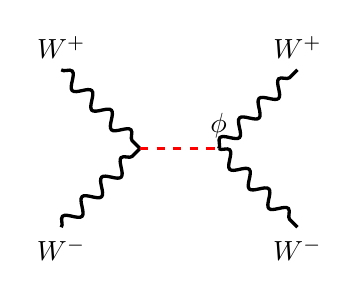
\begin{tikzpicture}
        % 

        % Draw the quarks
        \draw[boson] (0,0) node[left,below] {$W^{-}$} -- (1,1)  ;
        \draw[boson] (0,2) node[left,above] {$W^{+}$} -- (1,1)  ;

        \draw[higgs] (1,1) -- (2,1) node[above] {$\phi$} ;

        \draw[boson] (2,1) -- (3,2) node[right,above] {$W^{+}$} ;
        \draw[boson] (2,1) -- (3,0) node[right,below] {$W^{-}$} ;

    \end{tikzpicture}

\end{document} 



